\documentclass[11pt, a4paper]{article}

\usepackage[french]{babel}

\usepackage[utf8]{inputenc}
\usepackage[T1]{fontenc}

\usepackage{xcolor}

\usepackage{amsmath}
\usepackage{amssymb}
\usepackage{amsfonts}
\usepackage{eurosym}

\usepackage{graphicx}

\usepackage{tikz}

\usepackage{hyperref}
\hypersetup{
    colorlinks=true,
    linkcolor=red,
    }

\usepackage[]{geometry}
\setlength{\parindent}{0cm}
\setlength{\parskip}{.5\baselineskip}
\linespread{1.3}


\begin{document}

    \section*{Économétrie 101}

    \textit{Ce document présente un traitement informel du modèle causal de Rubin et des
    méthodes d'économétrie. Deux références sur le sujet sont \textit{Mastering
    Metrics} et \textit{Mostly Harmless Econometrics}, de J.\ Angrist et J.-S.\
    Pischke.}

    La plupart des travaux empiriques d'économie cherchent à mesurer l'effet
    que cause une variable (que l'on nomme \textit{traitement}) sur une autre (que l'on
    appelle généralement \textit{variable d'intérêt}).

    Qu'entend-on par \textit{effet du traitement} ? Il s'agit de la différence
    du niveau de la variable d'intérêt avec ou sans traitement, toutes choses
    égales par ailleurs.

    Par exemple (chiffres fictifs) si le taux de chômage à Trantor est de
    10\% avec une semaine de travail  de 35 heures alors qu'il aurait été de 8\% avec une semaine de travail de
    39 heures, l'effet du traitement \og{}passer d'une durée de la semaine de
    travail de 39 heures à 35 heures\fg{}sur la variable d'intérêt \og{}taux
    de chômage\fg{} est de \(10\% - 8\% =  2\) points de pourcentage.

    Soit \(T_{\text{Trantor}}\) une variable qui est égale à 1 si la Trantor est
    \og{}traitée\fg{} (dans notre exemple, passage aux 35 heures) et 0 si elle
    ne l'est pas.

    On note \(Y_{\text{Trantor}}\) notre variable d'intérêt. Elle peut prendre deux
    valeurs possibles : \(Y_{\text{Trantor}}\left(1\right)\),
    si  \(T_{\text{Trantor}} = 1\) et \(Y_{\text{Trantor}}\left(0\right)\),
    si  \(T_{\text{Trantor}} = 0\).
    
    Autrement dit,
    \[ Y_{\text{Trantor}} = \begin{cases}
        Y_{\text{Trantor}}\left(1\right) & \text{si }  T_{\text{Trantor}} = 1 \\
        Y_{\text{Trantor}}\left(0\right) & \text{si }  T_{\text{Trantor}} = 0 
        \end{cases}
    \]

    Dans notre exemple,
    \[ Y_{\text{Trantor}}\left(1\right) = 10 \% \]
    \[ Y_{\text{Trantor}}\left(0\right) = 8 \% \]
    \[ Y_{\text{Trantor}} = Y_{\text{Trantor}}\left(1\right) = 10 \% \]


    L'effet causal \(\Delta\) du traitement est donc :
    \[ \Delta_{\text{Trantor}} = Y_{\text{Trantor}}\left(1\right) -
    Y_{\text{Trantor}}\left(0\right) \]

    Ou plus généralement, pour une observation \(i\) :
    \[ \Delta_{i} = Y_{i}\left(1\right) -
    Y_{i}\left(0\right) \]

    Est-il possible de mesurer à la fois \(Y_{\text{Trantor}}\left(1\right) \)
    et \(Y_{\text{Trantor}}\left(0\right)\) ?

    Non : il n'est possible de mesurer que des évènements qui se sont
    effectivement réalisés.

    Soit \(T_{\text{Trantor}} = 1\) et il est possible d'observer
    \(Y_{\text{Trantor}}\left(1\right)\) mais pas
    \(Y_{\text{Trantor}}\left(0\right)\) ; soit
    \(T_{\text{Trantor}} = 0\) et il est possible d'observer
    \(Y_{\text{Trantor}}\left(0\right)\) mais pas
    \(Y_{\text{Trantor}}\left(1\right)\).

    Quelque soit le statut du traitement (traité ou non traité), il manquera
    toujours la mesure du \textit{contrefactuel}, c'est à dire de l'évènement non
    réalisé pour calculer l'effet du traitement.

    \begin{table}[h]
        \begin{tabular}{|l|l|l|}
        \hline
        L'observation reçoit-elle le traitement ? & Réalité observable & Contrefactuel inobservable \\ \hline
        Oui : $T_{i} = 1$ & $Y_{i}\left(1\right)$ & $Y_{i}\left(0\right)$ \\ \hline
        Non : $T_{i} = 0$ & $Y_{i}\left(0\right)$ & $Y_{i}\left(1\right)$ \\ \hline
        \end{tabular}
    \end{table}

    Implicitement ou explicitement, toute calcul d'effet de traitement (tel que
    défini dans ce document) repose sur des hypothèses faites sur le ou les contrefactuels.

    Pour reprendre notre exemple, une première solution à notre problème d'impossibilité
    de mesurer le contrefactuel \(Y_{\text{Trantor}}\left(0\right)\)
    serait de comparer Trantor à une autre région non traitée, i.e.\ dont la semaine de travail
    est de 39 heures, par exemple Helicon.

    On pourrait alors calculer 
        \begin{align*}
            \Delta' &= Y_{\text{Trantor}} - Y_{\text{Helicon}} \\
                    &= Y_{\text{Trantor}}\left(1\right) - Y_{\text{Helicon}}\left(0\right)
        \end{align*}

    Les deux grandeurs, \(Y_{\text{Helicon}}\left(0\right)\)
    et \(Y_{\text{Trantor}}\left(= 1\right)\) sont bien mesurables.
    
    Est-ce que \(\Delta' = \Delta\) ? Autrement dit, notre comparaison Helicon---Trantor
    permet-elle de mesurer l'effet du traitement à Trantor ?
    
    Non, car la différence
    entre les deux régions est composée à la fois de l'effet du traitement \textit{et}
    des différences éventuelles entre Helicon et Trantor qui ne sont pas liées au
    traitement. Il est tout à fait possible que, même en l'absence de traitement,
    les deux régions aient un taux de chômage différent.

    En effet,
        \begin{align*}
           & \Delta' = &
               Y_{\text{Trantor}}\left(T_{\text{Trantor}} = 1\right)
             - Y_{\text{Helicon}}\left(T_{\text{Helicon}} = 0\right) \\
         & = &  Y_{\text{Trantor}}\left(T_{\text{Trantor}} = 1\right) \\
         &  & - Y_{\text{Trantor}}\left(T_{\text{Trantor}} = 0\right)
             + Y_{\text{Trantor}}\left(T_{\text{Trantor}} = 0\right) \\
         &  & - Y_{\text{Helicon}}\left(T_{\text{Helicon}} = 0\right) \\
         & = &   \underbrace{\Delta}_{\text{Effet du traitement}}
             + \underbrace{Y_{\text{Trantor}}\left(T_{\text{Trantor}} = 0\right)
             - Y_{\text{Helicon}}\left(T_{\text{Helicon}} = 0\right)}_{\text{Différence entre Helicon et Trantor en l'absence de traitement}} \\
        \end{align*}

    Affirmer que \(\Delta' = \Delta\), c'est supposer qu'en l'absence de traitement à Trantor, Trantor et Helicon auraient le même taux de chômage, i.e.\ que l'on se trouve dans le cas particulier où \(Y_{\text{Trantor}}\left(0\right) - Y_{\text{Helicon}}\left(0\right) = 0 \Rightarrow Y_{\text{Trantor}}\left(0\right) = Y_{\text{Helicon}}\left(0\right) \). Cette hypothèse n'est pas directement vérifiable (puisque l'on ne peut observer 
    \(Y_{\text{Trantor}}\left(0\right)\)).
    
    Le même problème se retrouve lorsque l'on cherche à calculer un effet moyen du traitement sur un     ensemble d'observations. En notant \(\mathbf{E}\left[Y | X \right]\), la moyenne de \(Y\) pour
    le groupe \(X\), l'effet moyen du traitement (que l'on notera \(\boldsymbol{\Delta}\)) est :
    \begin{align*}
        \boldsymbol{\Delta} = \mathbf{E}\left[\Delta_{i} \right] &= \mathbf{E}\left[Y_{i}\left(1\right) - Y_{i}\left(0\right) \right] \\
                                       &= \mathbf{E}\left[Y_{i}\left(1\right)\right] - \mathbf{E}\left[Y_{i}\left(0\right) \right] \\
    \end{align*}
    
    Comme pour notre comparaison Trantor --- Helicon, on pourrait être tenté de comparer la moyenne de \(Y\) parmi les
    régions traitées à la moyenne des \(Y\) dans les régions non traitées. Cela permet-il de calculer l'effet moyen du traitement ?
    Non, pour la même raison que précédemment : les régions traitées et non traitées diffèrent certes du fait de l'effet du 
    traitement, mais peuvent également être différentes même en l'absence de traitement :
    
    \begin{align*}
        & \boldsymbol{\Delta'} = &
        \underbrace{\mathbf{E}\left[Y_{i} | T\left(i\right) = 1\right]}_{\text{Moyenne de la variable d'intérêt chez les traités}}   -  \underbrace{\mathbf{E}\left[Y_{i} | T\left(i\right) = 0\right]}_{\text{Moyenne de la variable d'intérêt chez les non traités}} \\
    & = &\underbrace{\mathbf{E}\left[Y_{i}\left(1\right) | T\left(i\right) = 1\right]}_{\text{Moyenne de la variable d'intérêt chez les traités}}   -  \underbrace{\mathbf{E}\left[Y_{i}\left(0\right) | T\left(i\right) = 0\right]}_{\text{Moyenne de la variable d'intérêt chez les non traités}} \\
        & = & \mathbf{E}\left[Y_{i}\left(1\right) | T\left(i\right) = 1\right]  \underbrace{- \mathbf{E}\left[Y_{i}\left(0\right) | T\left(i\right) = 1\right] + \mathbf{E}\left[Y_{i}\left(0\right) | T\left(i\right) = 1\right]}_{=0} - \mathbf{E}\left[Y_{i}\left(0\right) | T\left(i\right) = 0\right] \\
            & = & \underbrace{\mathbf{E}\left[Y_{i}\left(1\right) | T\left(i\right) = 1\right]  - \mathbf{E}\left[Y_{i}\left(0\right) | T\left(i\right) = 1\right]}_{=\boldsymbol{\Delta}} + \mathbf{E}\left[Y_{i}\left(0\right) | T\left(i\right) = 1\right] - \mathbf{E}\left[Y_{i}\left(0\right) | T\left(i\right) = 0\right] \\
        & = & \underbrace{\boldsymbol{\Delta}}_{\text{Effet du traitement}} + \underbrace{\mathbf{E}\left[Y_{i}\left(0\right) | T\left(i\right) = 1\right] - \mathbf{E}\left[Y_{i}\left(0\right) | T\left(i\right) = 0\right]}_{\text{Différence entre traités et non traités en l'absence de traitement}} 
    \end{align*}
    
    Une comparaison naïve entre régions traitées et régions non traitées ne
    permet pas de distinguer l'effet du traitement \(\boldsymbol{\Delta}\)
    des différences pré-existantes entre traités et non traités \(
    \mathbf{E}\left[Y_{i}\left(0\right) | T\left(i\right) = 1\right] - \mathbf{E}\left[Y_{i}\left(0\right) | T\left(i\right) = 0\right]\).

    En effet, si --- par exemple --- \(\boldsymbol{\Delta'} = 0.05\), comment
    savoir si :
    
    \begin{itemize}
        \item \(\boldsymbol{\Delta} = 0.03\) et \(
    \mathbf{E}\left[Y_{i}\left(0\right) | T\left(i\right) = 1\right] - \mathbf{E}\left[Y_{i}\left(0\right) | T\left(i\right) = 0\right] = 0.02\)
        \item ou si \(\boldsymbol{\Delta} = -0.04\) et \(
    \mathbf{E}\left[Y_{i}\left(0\right) | T\left(i\right) = 1\right] - \mathbf{E}\left[Y_{i}\left(0\right) | T\left(i\right) = 0\right] = 0.09\)
        \item ou encore \(\boldsymbol{\Delta} = 0\) et \(
    \mathbf{E}\left[Y_{i}\left(0\right) | T\left(i\right) = 1\right] - \mathbf{E}\left[Y_{i}\left(0\right) | T\left(i\right) = 0\right] = 0.05\) ?

    \end{itemize}
    
    Il faut à nouveau supposer que \(\mathbf{E}\left[Y_{i}\left(0\right) | T\left(i\right) = 1\right] - \mathbf{E}\left[Y_{i}\left(0\right) | T\left(i\right) = 0\right] = 0\). Hypothèse tout aussi invérifiable que précédemment (si \(T\left(i\right) = 1\), alors \(Y_{i} = Y_{i}\left(1\right)\) et \(Y_{i}\left(0\right)\) 
    n'est pas observé et donc \( \mathbf{E}\left[Y_{i}\left(0\right) | T\left(i\right) = 1\right] = 0\) non plus).
    
    Dans quel cas l'hypothèse  \(\mathbf{E}\left[Y_{i}\left(0\right) | T\left(i\right) = 1\right] - \mathbf{E}\left[Y_{i}\left(0\right) | T\left(i\right) = 0\right] = 0\) n'est-elle pas aberrante ?
    
    
    
    
    
\end{document}

    \frametitle{Point méthodologie : la différence de différence}
        \begin{itemize}
        \item Notations
            \begin{itemize}
                \item $Y_{i,t}$ : variable d'intérêt, dont la valeur
                    dépend de l'unité observée $i$ et de la période $t$
                \item $Y_{0,i,t}$ : valeur en l'absence du traitement (la réforme)
                \item $Y_{1,i,t}$ : valeur si il y a traitement
                \item Effet du traitement :  $Y_{1,i,t} - Y_{0,i,t}$
                \item Par définition, on ne peut observer $Y_{1,i,t}$
                    et  $Y_{0,i,t}$ en même temps !
                \item On appelle ``contrefactuel" la valeur non-observée :
                    \begin{itemize}
                        \item $Y_{1,i,t}$ pour les observations
                            \textbf{non}-traitées
                        \item $Y_{0,i,t}$ pour les observations traitées
                \end{itemize}
            \end{itemize}
        \item Cas de la réforme du New Jersey : on observe \dots
            \begin{itemize}
                \item $Y_{0,NJ,t}$
                \item $Y_{1,NJ,t+1}$
                \item $Y_{0,PA,t}$
                \item $Y_{0,PA,t+1}$
            \end{itemize}
        \item Manque le contrefactuel $Y_{0,NJ,t+1}$
        \end{itemize}
\end{frame}


\begin{frame}{DiD}

    \begin{figure}
        \includegraphics[scale=0.4]{figures/graphe_observe}
    \end{figure}

\end{frame}

\begin{frame}{DiD}
    \begin{figure}
        \includegraphics[scale=0.4]{figures/graphe_contrefactuel}
    \end{figure}
\end{frame}

\begin{frame}{DiD}
    \begin{figure}
        \includegraphics[scale=0.4]{figures/graphe_passe}
    \end{figure}
\end{frame}

\begin{frame}{DiD}
    \begin{figure}
        \includegraphics[scale=0.4]{figures/graphe_controle}
    \end{figure}
\end{frame}

\begin{frame}{DiD}
    \begin{figure}
        \includegraphics[scale=0.4]{figures/graphe_did}
    \end{figure}
\end{frame}

\begin{frame}{DiD}
    \begin{figure}
        \includegraphics[scale=0.4]{figures/graphe_final}
    \end{figure}
\end{frame}


\begin{frame}
    \frametitle{Point méthodologie : la différence de différence}
        On décompose la valeur de $Y$ en trois composantes :
        \begin{itemize}
            \item $\delta$ l'effet du traitement : $\delta = Y_{1,i} - Y_{0,i}$
            \item $\alpha_{t}$ la variation de $Y$ en $t$
            \item $\beta_{i}$ la variation de $Y$ en $i$
        \end{itemize}

        On observe \dots
        \begin{itemize}
        \item $Y_{1,NJ,t+1} = \alpha_{t+1} + \beta_{NJ} + \delta$
        \item $Y_{0,NJ,t} = \alpha_{t} + \beta_{NJ}$
        \item $Y_{0,PA,t} = \alpha_{t} + \beta_{PA}$
        \item $Y_{0,PA,t+1} = \alpha_{t+1} + \beta_{PA}$
        \end{itemize}

\end{frame}


\begin{frame}
    \frametitle{Point méthodologie : la différence de différence}
        Et on en déduit \dots
        \begin{align*}
            \alpha_{t+1} - \alpha_{t} &= \left(\alpha_{t+1} + \beta_{PA}\right) - \left(\alpha_{t} + \beta_{PA}\right) \\
            &= Y_{0,PA,t+1} - Y_{0,PA,t}
        \end{align*}

        \begin{align*}
            \delta + \alpha_{t+1} - \alpha_{t} &= \left(\alpha_{t+1} + \beta_{NJ} + \delta\right) - \left(\alpha_{t} + \beta_{NJ}\right) \\
            &= Y_{1,NJ,t+1} - Y_{0,NJ,t}
        \end{align*}

        \begin{align*}
            \delta &= \left(Y_{1,NJ,t+1} - Y_{0,NJ,t}\right) - \left( Y_{0,PA,t+1} - Y_{0,PA,t} \right)
        \end{align*}

\end{frame}


\begin{frame}
    \frametitle{Point méthodologie : la différence de différence}

        Hypothèse fondamentale :
        \begin{itemize}
            \item $\alpha_{t+1} - \alpha_{t}$ a la même valeur pour le groupe traité que pour le groupe de contrôle ("parallel trends")
            \item Si ce n'est pas le cas, on ne mesure plus $\delta$ mais $\delta + \left(\alpha_{NJ, t+1} - \alpha_{NJ, t}\right) - \left(\alpha_{PA, t+1} - \alpha_{PA, t}\right)$ \dots
        \end{itemize}

        Autres hypothèses :
        \begin{itemize}
            \item Traitement exogène
            \item Pas de contamination
            \item Pas d'attrition endogène
        \end{itemize}
\end{frame}

\begin{frame}
    \frametitle{Point méthodologie : la différence de différence}

        Retour à l'article :
        \begin{itemize}
            \item Quels effets mesurés ?
            \item Validité interne : est-ce que l'effet est bien mesuré ? Est ce que l'hypothèse des tendances parallèles est vérifée ?
            \item Validité externe : résultat généralisable à d'autres
                industries, périodes, pays, niveaux de salaire ?
                $\Rightarrow$ mesure d'un effet local
            \item Nécessaire de multiplier les évaluations
        \end{itemize}
\end{frame}

\begin{frame}{DiD}

    \begin{figure}
        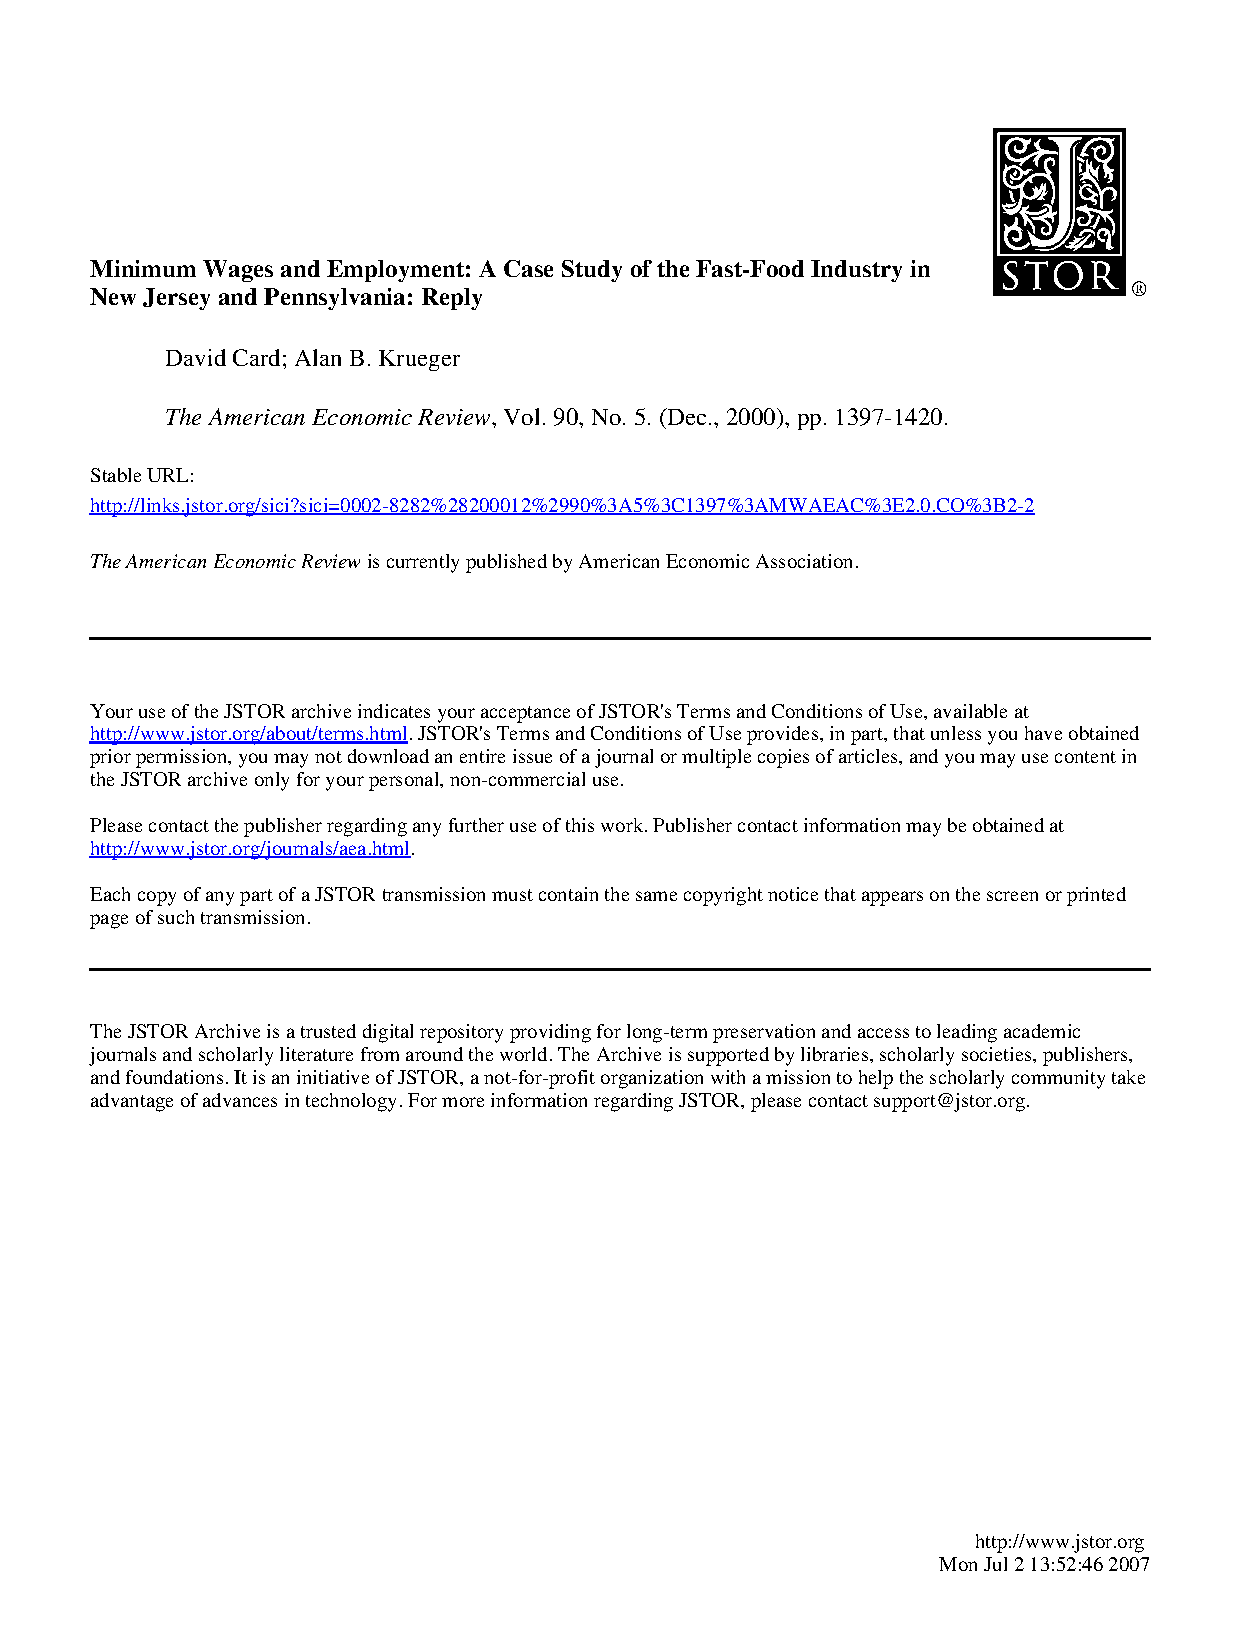
\includegraphics[scale=0.25]{figures/card_krueger_2000}
    \end{figure}

    {\small Source:Card \& Krueger (2000)}

\end{frame}


    \textbf{1.} En quoi consiste la méthode de régression sur discontinuité, utilisée
    dans l'article de Thomas Le Barbanchon (2016) ? Sous quelle hypothèse permet-elle
    d'identifier un effet causal ?

    Soit une valeur \(z^{*}\) dans une variable \(z\) telle que les individus soient traités
    si \(z_{i} \geq z^{*}\) et non traités si \(z_{i} < z^{*}\). La valeur \(z^{*}\) consistitue
    ainsi une discontinuité dans le niveau de traitement.
    
    Les individus de part et d'autres de la discontinuité sont très similaires en moyenne,
    puisqu'ils ont des valeurs de \(z\) quasiment identiques. Néanmoins, ils reçoivent des
    niveaux de traitement différents.
    
    Le groupe non traité d'un côté de la discontinuité peut ainsi servir de groupe de contrôle
    pour le groupe traité de l'autre côté de la discontinuité.

    L'hypothèse nécessaire est que toutes les autres caractéristiques, autres que le niveau de traitement,
    soient continues au niveau de la discontinuité ; ainsi, si l'on observe une discontinuité dans la
    variable d'intérêt \(y\), on peut l'attribuer à l'effet de la discontinuité dans le niveau de traitement, toutes les autres variables étant continues en ce point.
    
    Cette hypothèse n'est particulièrement pas vérifiée si les individus peuvent manipuler leur valeur
    de \(z\), i.e.\ choisir de quel côté de la discontinuité ils sont. Alors, les individus de
    part et d'autre de la discontinuité seront différents de manière discontinue sur au moins deux dimensions :
    \begin{itemize}
        \item le niveau de traitement
        \item la ou les variables qui expliquent que certains manipulent \(z\) et pas d'autres, par exemple être plus motivé ou mieux connaître le système socio-fiscal
    \end{itemize}
    
    Dans ce cas, il n'est pas possible de distinguer les deux effets.
    
    \dotfill
    
    \textbf{2.} En quoi diffère-t-elle de la méthode du bunching ?

    \dotfill
    
    Dans le cas d'une régression par discontinuité, on suppose que les individus ne peuvent pas manipuler
    leur position par rapport à la discontinuité en \(z\), qui détermine le niveau de traitement \(T\) dont
    on veut mesurer l'effet sur une variable \(y\). Autrement dit, on suppose que l'élasticité de \(z\)
    par rapport à \(T\) est nulle.
    
    Exemples : 
    \begin{itemize}
        \item \(z\) : Durée d'emploi
        \item \(T\) : Durée d'indemnisation du chômage
        \item \(y\) : Temps avant le retour à l'emploi
    \end{itemize}
    
    \begin{itemize}
        \item \(z\) : Taille de l'école
        \item \(T\) : Taille de la classe
        \item \(y\) : Résultats scolaires
    \end{itemize}
    
    \begin{center}
    \begin{tikzpicture}[scale=1.2]
    \node[] at (0,0) {$T$};
    \node[right] at (4,0) {$y$};
    \node[left] at (-4,0) {$z$};
    
    \node[above] at (2,0) {\begin{tabular}{c}Effet que l'on \\ cherche à mesurer\end{tabular}};
    \draw [->] (0.5, 0) -- (3.75, 0);
    
    \node[above] at (-2,0) {\begin{tabular}{c} Être à gauche ou à \\ droite de $z^{*}$ \end{tabular}};
    \draw [->] (-3.75, 0) -- (-0.5, 0);

    \node[below] at (0,-2) {$= 0$ par hypothèse};
    \draw [->] (3.75, -0.15) to[in = -45, out = -135] (-3.75, -0.15);
    \draw [->] (-0.25, -0.15) to[in = -45, out = -135] (-3.75, -0.15);

    \end{tikzpicture}
    \end{center}
    
    Dans le cas du bunching, on cherche au contraire à déterminer la valeur de l'élasticité de \(z\) par
    rapport à \(T\), i.e.\ dans quelle mesure les individus peuvent manipuler leur position. Cela implique que l'on ne peut pas mesurer l'effet de la discontinuité sur le niveau de traitement sur une autre
    variable \(y\), pour les raisons évoquées précédemment.
    
        \begin{center}
    \begin{tikzpicture}[scale=1.2]
    \node[] at (0,0) {$T$};
    \node[right] at (4,0) {$y$};
    \node[left] at (-4,0) {$z$};
    
    \node[above] at (2,0) {?};
    \draw [->] (0.5, 0) -- (3.75, 0);
    
    \node[above] at (-2,0) {Lien connu entre \(T\) et \(z\)};
    \draw [->] (-3.75, 0) -- (-0.5, 0);

    \node[below] at (-2,-1) {Réaction de \(z\) à \(T\) que l'on cherche à mesurer};
    \draw [->] (-0.25, -0.15) to[in = -45, out = -135] (-3.75, -0.15);
    \end{tikzpicture}
    \end{center}

    Exemple : 
    \begin{itemize}
        \item \(z\) : Salaire avant impôt
        \item \(T\) : Taux d'imposition
        \item \(y\) : Néant
    \end{itemize}

    \textbf{B.} \textit{4 points}

    \textbf{1.} En quoi consiste la méthode des variables instrumentales ?
    Quelles sont les conditions pour qu'un instrument soit valide ?

    \dotfill

    Afin d'estimer l'effet d'un traitement \(T\) sur une variable \(y\),
    faire une simple comparaison des individus traités et non traités n'est
    pas suffisant. En effet, si le traitement n'est pas alloué de manière aléatoire,
    cette comparaison mesure l'effet du traitement et la différence
    de composition entre le groupe traité et le groupe non traité.
    
    Il est possible de comparer deux groupes qui diffèrent selon une variable
    \(z\), que l'on appelle \textit{instrument}, telle que :
    \begin{itemize}
        \item Comparer ces deux groupes permet de comparer des individus
            qui n'ont pas le niveau de traitement ; autrement dit, l'instrument
            détermine le niveau de traitement. Cette caractéristique
            est parfois appelée condition de pertinence.
        \item Les individus des deux groupes ont les mêmes contrefactuels ;
            autrement dit, il n'y a pas de différence inobservée de composition entre
            les deux groupes ; dit encore d'une autre façon, la seule manière
            dont le niveau de traitement affecte la variable \(y\) est via son
            effet sur le traitement \(T\). Cette condition est appelée condition
            d'exclusion. Cette hypothèse n'est pas directement vérifiable empiriquement.
    \end{itemize}

    Il est possible de représenter ces conditions par une chaîne causale, où
    une flèche entre \(A\) et \(B\) indique que \(A\) cause \(B\).
    
    La relation que l'on cherche à estimer est la suivante :
    \begin{center}
    \begin{tikzpicture}[scale=1.2]
    \node[] at (0,0) {T};
    \node[] at (2,0) {y};
    \node[above] at (1,0) {?};

    \draw [->] (0.25, 0) -- (1.75, 0);
    \end{tikzpicture}
    \end{center}
    
    Néanmoins, on ne peut exclure que le niveau de la variable d'intérêt détermine
    le niveau de traitement (probabilité de causalité inverse : par exemple, les
    mauvais étudiants peuvent être placés dans des classes plus petites) ou
    qu'une autre variable détermine à la fois le niveau de traitement et
    le niveau de \(y\).
    
    \begin{center}
    \begin{tikzpicture}[scale=1.2]
    \node[] at (0,0) {T};
    \node[] at (2,0) {y};
    \node[] at (1,-1.5) {x};
    
    \node[above] at (1,0.35) {?};
    \draw [->] (0.25, 0.05) to[in = 135, out = 45] (1.75, 0.05) ;
    
    \node[below] at (1,-0.35) {?};
    \draw [->] (1.75, -0.05) to[in = -45, out = -135] (0.25, -0.05);

    \draw [->] (0.75, -1.5) to[in = -90, out = 180] (0, -0.25);
    \draw [->] (1.25, -1.5) to[in = -90, out = 0] (2, -0.25);
    \node[left] at (1.9,-1) {?};
    \node[right] at (0.1,-1) {?};
    
    \end{tikzpicture}
    \end{center}

    L'instrument permet d'isoler une seule de ces (possibles) chaînes causales :
    
    \begin{center}
    \begin{tikzpicture}[scale=1.2]
    \node[] at (0,0) {T};
    \node[] at (2,0) {y};
    \node[] at (-2,0) {z};
    
    \node[above] at (1,0) {?};
    \draw [->] (0.25, 0) -- (1.75, 0);
    
    \node[above] at (-1,0) {$\neq 0$};
    \draw [->] (-1.75, 0) -- (-0.25, 0);

    \node[below] at (0,-1) {$= 0$ par hypothèse};
    \draw [->] (1.75, -0.05) to[in = -45, out = -135] (-1.75, -0.05);

    \end{tikzpicture}
    \end{center}

    Prenons un exemple plus concret :
    \begin{itemize}
        \item \(z\) : être assigné aléatoirement par le chercheur dans le groupe de traitement 
        \item \(T\) : le traitement
        \item \(y\) : la variable d'intérêt
    \end{itemize}
    
    Dans ce cas de l'expérience randomisé, l'instrument a un effet sur le niveau de traitement ;
 cet effet n'est pas nécessairement \og{}parfait\fg{} si certains individus sont assignés au groupe de traitement mais n'en bénéficient pas.
    Aucune variable n'influe à la fois sur l'instrument et sur la variable d'intérêt,
    puisque l'instrument est aléatoire. La variable d'intérêt
    n'influe pas sur l'instrument puisqu'il est complètement aléatoire.
    
    Prenons un cas plus litigieux mais classique en économie du développement :
    dans quelle mesure les crises économiques causent des crises politiques ou
    l'inverse, et dans quelle mesure ?

    Comparer naïvement des pays en crise politique aux autres et observer qu'ils
    ont une moins bonne performance économique ne permet pas de déterminer si
    les crises politiques causent des crises économiques, l'inverse ou les deux.
    
    Une solution possible est de comparer les observations (par exemple, un pays un mois donné) qui subissent des évènements météorologiques extrêmes (sécheresse,
    inondations) à ceux qui n'en subissent pas. La seule différence entre ces
    deux groupes est que les premiers seront en crise économique pour une cause
    exogène (la météo) et pas les autres. Comparer les premiers au seconds permet
    de déterminer l'effet d'une crise économique \textit{qui n'est pas causée par
    une crise politique, ni pas une autre caractéristique sous-jacente} sur la
    stabilité politique. On peut exclure que l'effet trouvé soit la causalité 
    inverse, puisque cela supposerait que les crises politiques causent des
    évènements météorologiques extrêmes, ce qui est absurde (à court terme du moins).
    
        \begin{itemize}
        \item \(z\) : météo extrême
        \item \(T\) : situation économique
        \item \(y\) : situation politique
    \end{itemize}

    \begin{center}
    \begin{tikzpicture}[scale=1.2]
    \node[] at (0,0) {\begin{tabular}{c}Crise  \\ économique\end{tabular}};
    \node[right] at (4,0) {Situation politique};
    \node[left] at (-4,0) {Météo extrême};
    
    \node[above] at (2,0) {\begin{tabular}{c} Effet de l'économie sur \\ la situation politique \end{tabular}};
    \draw [->] (0.5, 0) -- (3.75, 0);
    
    \node[above] at (-2,0) {\begin{tabular}{c} Effet de la météo \\ sur l'économie \end{tabular}};
    \draw [->] (-3.75, 0) -- (-0.5, 0);

    \node[below] at (0,-2) {Effet de la situation politique sur la météo  $= 0$ par hypothèse};
    \draw [->] (3.75, -0.15) to[in = -45, out = -135] (-3.75, -0.15);

    \end{tikzpicture}
    \end{center}

    Il est alors possible de mesurer :
    \begin{itemize}
        \item L'effet de la météo extrême sur la situation politique
        \item L'effet de la météo extrême sur l'économie
    \end{itemize}
    
    Puisque l'on a supposé que l'effet de la météo extrême sur
    la situation politique n'a lieu qu'à travers son effet sur l'économie, on a :
    effet de la météo extrême sur la situation politique $=$ effet de la météo extrême sur l'économie $\times$ effet de l'économie sur la situation politique ;
    et donc : \[ \text{{\small effet de l'économie sur la situation politique }} = \frac{\text{{\small effet de la météo extrême sur la situation politique}}}{\text{{\small effet de la météo extrême sur l'économie}}} \]
    
    Intuitivement, l'instrument correspond à de la variation exogène dans le niveau de traitement.
    
    Un point à garder en tête est que, puisque l'on n'utilise que la variation
    dans le traitement causée par l'instrument, on estime un effet causal
    sur les individus pour qui l'instrument a un effet (les \og{}compliers\fg{}),
    une population potentiellement particulière.

    \dotfill

    \textbf{2.} Les instruments utilisés dans les trois articles des exposés
    satisfont-ils ces conditions ?

    \textbf{Lleras-Muney}. La situation est la suivante :
        \begin{itemize}
        \item \(z\) : lois sur l'éducation
        \item \(T\) : niveau d'éducation
        \item \(y\) : santé
    \end{itemize}

    Pour que l'instrument soit valide, il faut qu'il ait un effet sur le niveau
    d'éducation, ce qui est ici le cas (on peut imaginer qu'il n'y a pas d'effet si
    les lois ne sont pas contraignantes, i.e. que tout le monde étudie plus que
    la durée minimale et donc que les lois n'aient pas d'effet sur le niveau
    d'éducation).
    
    Par ailleurs, il faut que le niveau de santé de la population n'influe pas sur
    les réformes éducatives (par exemple, que les députés ne décident pas d'augmenter
    le niveau minimal d'éducation obligatoire parce qu'ils constatent une crise sanitaire), ni qu'une tierce variable n'affecte à la foi les lois sur l'éducation et la santé des individus (par exemple, que, face à une crise économique, la santé des individus se dégrade et que les députés décident de réhausser l'âge de la fin de l'éducation obligatoire pour lutter contre cette crise).
    
    \textbf{Angrist et Lavy}. La situation est la suivante :
        \begin{itemize}
        \item \(z\) : Taille de l'école, ou plus exactement, distance aux seuils de la règle de Maïmonide
        \item \(T\) : Taille des classes
        \item \(y\) : Réussite scolaire
    \end{itemize}

    L'effet de la taille de l'école sur la taille des classes est très clair,
    via la règle de Maïmonide, bien qu'elle soit imparfaitement respectée.
    
    La condition d'exclusion serait violée si, par exemple, certains parents
    choisissaient de placer leurs enfants juste au dessus des discontinuités
    afin de leur garantir des petites classes. Néanmoins, les auteurs affirment
    que cette hypothèse est peu probable puisque la taille de l'école ne peut
    être connue avec précision avant la rentée ; qu'il y a peu d'alternatives à
    l'école publique si les enfants tombent dans une classe \og{}trop grande\fg{},
    et qu'il n'est pas possible de changer d'école publique sans déménager.
    
    \textbf{Aufhammer et Rubin}. La situation est la suivante :
        \begin{itemize}
        \item \(z\) : Prix de gros du gaz en Louisianne deux mois avant
        \item \(T\) : Prix à la consommation du gaz
        \item \(y\) : Consommation de gaz
    \end{itemize}

    Le prix de gros du gaz est répercuté par des règles connues sur le prix
    à la consommation et a effectivement un effet sur les prix à la consommation.
    
    La condition d'exclusion serait violée si, par exemple, la consommation de gaz
    en Californie avait un effet sur le prix de gros du gaz deux mois avant, ce qui
    paraît peu probable.
    
    Les questions suivantes portent sur Bozio, Irac et Py (2014).

    \textbf{0.} En quoi consistent les méthodes d'appariement (matching) ?

    \textbf{1.} Quelle est la stratégie d'identification utilisée par les
    auteurs ? Vous paraît-elle crédible ?

    \textbf{2.} Quel est l'effet estimé du \textsc{cir} sur les dépenses de
    recherche et développement ? Quel est l'effet estimé sur l'innovation ?
    Comment expliquez vous la différence entre ces deux effets ?

    \textbf{0.} En quoi consistent les méthodes d'appariement (matching) ?

    \dotfill

    Les groupes traités et non-traités ne sont pas nécessairement comparables,
    parce qu'ils diffèrent sur d'autres dimensions que l'assignation au traitement.

    Les méthodes d'appariement consistent à appareiller chaque membre du groupe
    traités avec un membre du groupe non-traités avec lequel ils partagent les
    mêmes caractéristiques observables.

    Il n'y a donc plus de biais de sélection sur les variables \textit{observables}.

    \dotfill

    \textbf{1.} Quelle est la stratégie d'identification utilisée par les
    auteurs ? Vous paraît-elle crédible ?

    \dotfill

    Les auteurs utilisent une méthode différence de différences, utilisant les entreprises
    bénéficiant du crédit d'impôt comme groupe traité et des entreprises similaires mais non
    traitées (cf. paragraphe sur l'appariement) comme groupe de contrôle. On suppose donc
    qu'en l'absence de demande du \textsc{cir} par les entreprises du premier groupe, celles-ci
    auraient évolué de la même manière que celles du second.

    Il paraît cependant probables que deux entreprises similaires pour tout ce qui est observable
    mais dont l'une choisit de demander le \textsc{cir} et pas l'autre, diffèrent
    sur des caractéristiques non observables. On peut par exemple supposer que les entreprises
    demandant le \textsc{cir} connaîssent mieux l'environnement légal du soutien public
    à l'innovation que les autres. Dans ce cas là, 
    l'hypothèse de tendances parallèles est peu crédible.   

    \dotfill

    \textbf{2.} Quel est l'effet estimé du \textsc{cir} sur les dépenses de
    recherche et développement ? Quel est l'effet estimé sur l'innovation ?
    Comment expliquez vous la différence entre ces deux effets ?

    \dotfill

    Le \textsc{cir} augmente de manière importante les dépenses de recherche
    et développement sans pour autant augmenter le nombre de brevets déposés.

    Cela provient soit d'un réétiquetage de dépenses autres en dépenses de recherche
    et développement pour bénéficier du \textsc{cir} sans faire davantage de recherche ;
    soit que la mesure de l'innovation n'est pas bonne, notamment parce qu'il n'y a pas
    assez de recul pour que l'innovation supplémentaire --- si il y en a eu --- se traduise
    en brevets.
 
    \dotfill

    \textbf{1.} En quoi consiste la méthode de \og bunching\fg{} utilisée dans
    l'article \og Migration and wage effects of taxing top earners \fg{} de
    Kleven et al (Quarterly Journal of Economics, 2014) ?


    On peut supposer que la distribution des revenus en l'absence de système
    socio-fiscal est \og lisse \fg{}, c'est à dire sans trou ou accumulation en
    un point. Un système socio-fiscal non linéaire, c'est à dire avec des
    discontinuités dans le taux marginal d'imposition (kinks) ou dans le taux
    moyen d'imposition (notches) fournit des incitations à s'agglomérer à ces
    points de non linéarités. Par exemple, les individus éligibles au dispositif
    fiscal danois étudié ont une incitation très forte à gagner au moins un
    million d'euros pour bénéficier de la discontinuité dans le taux moyen
    d'imposition à ce seuil.

    Le volume de ces accumulations aux seuils dépend de la réaction des agents
    aux non-linéarités du système socio-fiscal. Si les agents sont parfaitement
    inélastiques à la taxation, une non linéarité ne modifiera pas leur
    comportement et donc la distribution des revenus. Au contraite, si les
    revenus des agents sont très élastiques à la taxation, ils auront tendance à
    tous s'accumuler aux seuils avantageux (\og bunch \fg{}).

    Ainsi en mettant en regard la taille des accumulations (c'est à dire
    \(\Delta\) revenu) avec la taille de la discontinuité (c'est \(\Delta\) taux
    d'imposition), on peut estimer l'élasticité du revenu à la taxation (c'est à
    dire \( \frac{\text{taxe}}{\text{revenu}} \frac{\Delta \text{ revenu}}{\Delta \text{ taxe}} \)).

    \textbf{B. DiD}

    Soient deux États A et B dont on observe le niveau de consommation tous les deux ans :
    \begin{table}[h!]
        \centering
        \begin{tabular}{c|cc}
        Année & État A & État B \\ \hline
        1994  & 100    & 90     \\
        1996  & 110    & 120    \\
        1998  & 130    & 130    \\
        2000  & 140    & 150
        \end{tabular}
        \caption{Niveau de consommation par année et par État}
    \end{table}

    En 1997, l'État A implémente une baisse de la \textsc{tva}. L'État B ne modifie pas son système socio-fiscal sur la période.
    On cherche à estimer l'effet causal de cette baisse de la \textsc{tva} sur le niveau de consommation.

    \textbf{1.} Calculez l'effet estimé de la baisse de \textsc{tva} par la méthode de la différence de différences.

    \textbf{2.} Calculez le même estimateur entre 1996 et 1994. Quel résultat trouvez-vous ? Quel est le résultat attendu ?
    Qu'en concluez vous sur la validité de l'hypothèse nécessaire à l'utilisation de la méthode DiD ?
    \textbf{B. DiD}

    Soient deux États A et B dont on observe le niveau de consommation tous les deux ans :
    \begin{table}[h!]
        \centering
        \begin{tabular}{c|cc}
        Année & État A & État B \\ \hline
        1994  & 100    & 90     \\
        1996  & 110    & 120    \\
        1998  & 130    & 130    \\
        2000  & 140    & 150
        \end{tabular}
        \caption{Niveau de consommation par année et par État}
    \end{table}

    En 1997, l'État A implémente une baisse de la \textsc{tva}. L'État B ne modifie pas son système socio-fiscal sur la période.
    On cherche à estimer l'effet causal de cette baisse de la \textsc{tva} sur le niveau de consommation.

    \textbf{1.} Calculez l'effet estimé de la baisse de \textsc{tva} par la méthode de la différence de différences.

    \dotfill

    \(\hat{\delta} = \left( C_{A, 1998} - C_{A, 1996} \right) - \left( C_{B, 1998} - C_{B, 1996} \right) = 10\).

    \dotfill

    \textbf{2.} Calculez le même estimateur entre 1996 et 1994. Quel résultat trouvez-vous ? Quel est le résultat attendu ?
    Qu'en concluez vous sur la validité de l'hypothèse nécessaire à l'utilisation de la méthode DiD ?

    \dotfill

    \(\hat{\delta} = \left( C_{A, 1996} - C_{A, 1994} \right) - \left( C_{B, 1996} - C_{B, 1994} \right) = - 20\).

    L'effet de traitement attendu lorsqu'il n'y a pas de traitement est de 0 : or notre estimateur est de -20. C'est donc
    qu'il ne mesure pas correctement l'effet réel de traitement. 

    En l'absence de traitement, l'effet mesuré par l'estimateur DiD est :
    \[\left(\alpha_{A, 1996} - \alpha_{A, 1994} \right) - \left(\alpha_{B, 1996} - \alpha_{B, 1994} \right) \neq 0\]

    L'hypothèse des tendances parallèles n'est donc pas vérifiée entre 1994 et 1996 (ni entre 1998 et 2000).
    Il paraît donc douteux qu'elle le soit entre 1996 et 1998.

    \dotfill

